\section{IMU基本模型}

IMU是测量物体三轴角速度以及加速度的装置,包含三轴陀螺仪和线加速度计。IMU工作极其稳定,几乎不会有宕机的情况,而且通常能以远高于相机的频率(数百到上千赫兹)得到相对于自身坐标系的角速度$\bm{\omega}$($rad \cdot s^{-1}$)和加速度$\bm{a}$($m \cdot s^{-2}$)。依靠这些数据,可以通过数值积分计算得到系统的朝向$\mathrm{R}\in\mathbb{SO}^3$、速度$\bm{v}\in\mathbb{R}^3$和平移$\bm{l}\in\mathbb{R}^3$信息,因此基于IMU的跟踪结果直接就带有了场景的尺度信息。很自然地,IMU工作并不依赖于视觉信息,可以在相机遭遇恶劣的光照、纹理以及运动模糊的情况下提供较为可靠的跟踪结果。但值得注意的是,消费级别的IMU传感器,其信号通常带有较大的bias\footnote{指IMU输出值和输入值之间的偏移,可能受温度、重力等因素的影响}和噪声,并且系统的速度$\bm{v}$和平移$\bm{l}$分别来自于加速度$\bm{a}$的一次和二次数值积分,bias和噪声也会通过积分以平方级别被放大,带入到跟踪结果中。因此仅使用IMU的跟踪结果是不可靠的,需要定期使用视觉跟踪信息来纠正IMU跟踪的误差。

鉴于其噪声特性,合理地使用IMU辅助视觉跟踪是一项重大挑战。不管是使用滤波的方法还是非线性优化的方法融合视觉信息和IMU信息,都要对IMU的误差进行合理的建模。将IMU的实际物理运动定义为传感器的输入,IMU对实际运动进行测量得到角速度和加速度定义为传感器输出,则输出和输入的差异即为IMU读数的误差,常见的IMU误差模型可以用图~\ref{fig:common_imu_errors}来表示。

\begin{figure}[htb!]
    \centering
    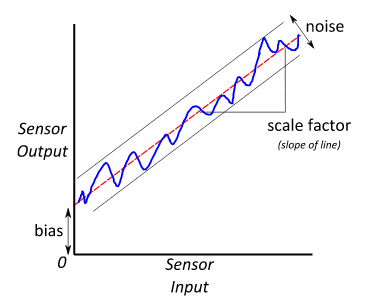
\includegraphics[width=.4\textwidth]{Pictures/common_imu_errors.png}
    \setcitestyle{sort&compress,longnamesfirst,square,numbers}
    \caption{一般的IMU误差模型\citep{imu2014}}
    \label{fig:common_imu_errors}
\end{figure}

可以看到,IMU误差的成分是比较复杂的,可能包含bias、随机游走噪声(random walk)\footnote{指当输入固定时,IMU输出值中包含的随机噪声,它随时间的变化可被认为是一个随机过程}、尺度系数(scale factor)\footnote{指的是输出和输入之间的线性缩放系数}、不正交性(non-orthogonality)\footnote{指由于IMU各轴并不完全正交所带来的误差}等等\citep{imu2014},而不同类型误差对于运动估计的影响也是不同的。在跟踪的过程中,系统的朝向$\mathrm{R}$可以通过角速度$\bm{\omega}$的数值积分得到;加速度$\bm{a}$会被进行一次和二次积分,分别得到速度$\bm{v}$和平移$\bm{l}$。加速度经过了二次数值积分,其误差也会通过两次积分进入平移量$\bm{l}$中,故相比角速度的误差,跟踪算法对于加速度的误差更为敏感。实际经验也表明,由IMU积分得到的朝向信息是较为准确的,而位置信息的误差则是较大的。

一般IMU在出厂时都会经过厂商的校准,故在实际跟踪和状态估计的过程中可以使用一个简化的IMU误差模型。以常用的六轴IMU为例,
大部分的VISLAM系统都使用了相同的IMU误差模型,如MSCKF、VINS-Mono等,即将其误差简化为bias和测量噪声两个部分,并假设加速度计和陀螺仪相互统计独立,且各自的三轴之间都统计独立。使用下标$m$标记每次测量的值,不带下标的表示真实值左上标$^G$来表示参考系为全局坐标系,不带左上标的表示参考系为局部坐标系。在不考虑地球自转的情况下,角速度和加速度的测量分别为:
\begin{equation}
\begin{aligned}
    \tilde{\bm{\omega}}
        &= \bm{\omega} + \bm{b}^g + \bm{n}^g,  \\
    \tilde{\bm a}
        &= \prescript{G}{}{\mathrm{R}^\top}
            (\prescript{G}{}{\bm a} - \prescript{G}{}{\bm{g}}) +
                \bm{b}^a + \bm{n}^a
\end{aligned}
\end{equation}
可以看到,IMU的的读数可以看成是真实值、偏移和加性高斯白噪声(addative Gaussian white noise)之和。而加速度的测量中又包含了重力$\prescript{G}{}{\bm g}$的影响。bias和白噪声具备如下性质:
\begin{itemize}
    \item bias~$\bm{b}^g$和$\bm{b}^a$:随时间的增长符合零均值的高斯随机游走。该噪声从IMU开机以来就一直存在,不断积累,与是否从IMU读取数据无关。可以用如下高斯分布来描述:
        \begin{equation}
        \begin{aligned}
            \bm{b}^g &\sim \mathcal{N}(\bm{b}_0^g, \mathrm{Q}_g), \\
            \bm{b}^a &\sim \mathcal{N}(\bm{b}_0^a, \mathrm{Q}_a)
        \end{aligned}
        \end{equation}
    \item 测量噪声$\bm{n}^g$和$\bm{n}^a$:零均值加性高斯白噪声,表示从IMU读取数据时产生的小抖动,而且这个噪声只在测量时产生,也符合高斯分布:
        \begin{equation}
        \begin{aligned}
            \bm{n}^g & \sim \mathcal{N}(\bm{0}, \mathrm{R}_g), \\
            \bm{n}^a & \sim \mathcal{N}(\bm{0}, \mathrm{R}_a),
        \end{aligned}
        \end{equation}
\end{itemize}
为了方便后续的计算,IMU测量误差的协方差也可以记为:
\begin{equation}
\Sigma =
    \begin{bmatrix}
        \mathrm{Q}_g &            0 &            0 &         0 \\
                   0 & \mathrm{R}_g &            0 &         0 \\
                   0 &            0 & \mathrm{Q}_a &         0 \\
                   0 &            0 &            0 & \mathrm{R}_a
    \end{bmatrix}
\end{equation}

\subsection{离散时间噪声和连续时间噪声}

上面提到的噪声模型都是在连续时间系统下面考虑的,连续时间系统的高斯协方差(或标准差)也就称为传感器的噪声强度。实际应用中,不可能每时每刻都在读取IMU数据,而应该考虑离散时间系统的情况。\citep{smith1978exact}给出了离散时间噪声和连续时间噪声的关系。可知,离散时间系统下IMU噪声的协方差与连续时间系统存在如下关系:
\begin{equation}
\begin{aligned}
    \mathrm{Q}_{gd} &= \mathrm{Q}_g \Delta t   \\
    \mathrm{Q}_{ad} &= \mathrm{Q}_a \Delta t   \\
    \mathrm{R}_{gd} &= \mathrm{R}_g / \Delta t \\
    \mathrm{R}_{ad} &= \mathrm{R}_a / \Delta t
\end{aligned}
\end{equation}
其中$\Delta t$为采样时间间隔,并且陀螺仪、加速度计三轴的噪声统计独立。

\subsection{IMU状态传播}

所谓的IMU状态传播(IMU propagation)指的就是根据通过将当前时刻IMU的读数在时间上进行积分,来得到下一时刻的IMU状态。这个IMU状态包括IMU的位姿、运动以及噪声等,通过积分操作,IMU读数的信息就被传播到了下一时刻。

首先考虑理想情况,也就是IMU的读数不存在白噪声,偏移量也不存在随机游走的情况,此时IMU的读数符合:
\begin{equation}
\begin{aligned}
    \bm{\omega}  &= \tilde{\bm{\omega}} - \bm{b}^g, \\
    \bm{a} &= \tilde{\bm a} - \bm{b}^a + \bm{g}.
\end{aligned}
\end{equation}

记全局坐标系下IMU的状态为(为保持简洁,省略了转置符号${}^\top$):

\begin{equation}
  \bm{X}_{\textrm{IMU}} \doteq
  \left[
      \prescript{G}{}{\mathrm R},
      \prescript{G}{}{\bm p},
      \prescript{G}{}{\bm v},
      \bm{b}^g, \bm{b}^a
  \right].
\end{equation}

具体来说,积分过程包括积分这个IMU状态向量的五个分量。那么,要对IMU状态进行积分,首先需要写出IMU状态关于时间的导数:
\begin{equation}
\begin{aligned}
    \prescript{G}{}{\dot{\mathrm R}}
        &= \prescript{G}{}{\mathrm R} \lfloor(\tilde{\bm{\omega}} - \bm{b}^g)\times\rfloor, \\
    \prescript{G}{}{\dot{\bm p}}
        &= \prescript{G}{}{\bm v}, \\
    \prescript{G}{}{\dot{\bm v}}
        &= \prescript{G}{}{\mathrm R} (\tilde{\bm a} - \bm{b}^a + \bm{g}), \\
    \dot{\bm b}^g &= \bm{0}, \\
    \dot{\bm b}^a &= \bm{0}
\end{aligned}
\end{equation}

显然,由于偏移$\bm{b}^g$和$\bm{b}^a$随时间的增长符合零均值的高斯随机游走,故它们关于时间的导数为零。积分的步骤如下:

\begin{enumerate}
    \item 将角速度在时间上积分,得到当前IMU的朝向;
    \item 将加速度在时间上积分,得到当前IMU的速度;
    \item 将速度再在时间上积分,得到当前IMU的位置;
    \item 角速度偏移和加速度偏移由于增长符合零均值随机游走,所以直接取旧的状态中的值。
\end{enumerate}

可以使用任意一种数值积分算法来实现,比如欧拉法(Euler method)、龙格库塔法(Runge-Kutta methods)等。此外,不仅要对状态向量进行数值积分,同时还要更新协方差矩阵。
